\chapter{Design and development\label{chap:design}}

\section{Open-Extension Container Structure\label{sec:design_oxc}}


Linux scheduling is runqueue, \texttt{struct rq}, centered and each 
scheduling class 
implements a set of interfaces to deal with the runqueue structure.
In mainline Linux, \texttt{struct rq} is a per CPU structure.
Each scheduling class defines its scheduling operations (enqueue, 
dequeue, etc.) with this per CPU runqueue. On Multiple processor
platform, tasks can migrate between different runqueues, also depending
on behaviours defined in specific scheduler.
In other words, on each CPU, a scheduling system is built up bsed on the
associated runqueue.
Different per CPU scheduling systems cooperate
with each other by task migrations defiend by specific scheduling class 
and construct the system level scheduling. 
The idea is that if there is one extra runqueue, each scheduler can still 
use it as scheduling parameter and a scheduling system can be built around 
it. If there are more than one extra runqueues, they can produce a pseudo 
system level scheduling system.   

Here a data structure named Open-Extension Container(OXC) is proposed,
shown in figure\ref{fig:oxc}.
\begin{figure}[htbp]
        \centering
        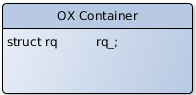
\includegraphics[width=0.5\textwidth]{images/oxc}
        \caption{Open-Extension Container}
        \label{fig:oxc}
\end{figure}
The ox container is designed as an abstract data structure; that is, any data
structure contains a \texttt{struct rq} runqueue inside can be called an ox
container. Now, in the system there is not only per CPU runqueues, but also 
per oxc runqueues.

\section{The oxc scheduling\label{sec:design_oxc_scheduling}}
As ox containers are defined, there are extra runqueues besides per CPU ones 
in a system. For each scheduler, they manage tasks above runqueues according
to implementation details in their scheduling class, and as long as a runqueue
parameter is provided for their schedulinf operations, they have do not care 
it is from a CPU or an ox container.
So as a oxc local runqueue is passed to hooks of scheduling classes, tasks would 
enqueue, operate and dequeue on a per container runqueue. As for tasks and scheduling
classes, there is no difference between a per CPU and per container runqueue.
This can be clearly shown when we see the scheduling scheme in the system 
with oxc scheduling. Recall the path which relates each
task with the per CPU runqueue it runs above in section \ref{sec:LinuxSched_cfs}
and \ref{sec:LinuxSched_rt}. Now let's see the scheduling scheme after the 
ox container joins the system with its local runqueue. 

From figure \ref{fig:oxc_fair_tg} and \ref{fig:oxc_rt_tg} we can see when 
task group scheduling is enabled, the scheduling route we saw before can also
lead a task to its per container runqueue. The same codes can still be used to
find both kinds of runqueues.

\begin{figure}[htbp]
\begin{center}
	\subfigure[cfs] {
        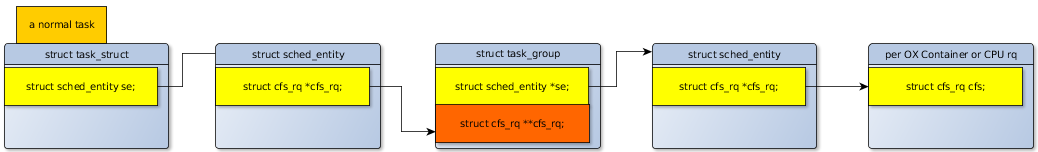
\includegraphics[height=2.5cm, width=\textwidth]{images/cfs_scheduling_scheme_tg_oxc}
        \label{fig:oxc_fair_tg}
	}
	\subfigure[rt] {
        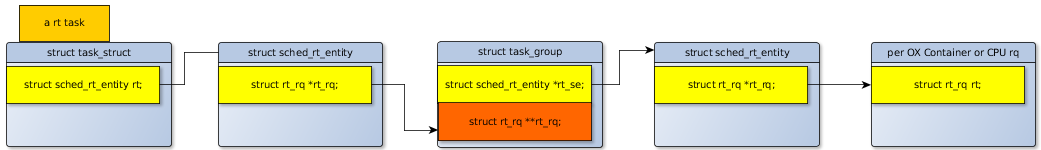
\includegraphics[height=2.5cm, width=\textwidth]{images/rt_scheduling_scheme_tg_oxc}
        \label{fig:oxc_rt_tg}
	}
\end{center}
	%\end{subfigure}
	\caption{Scheduling route with task group scheduling 
						in OXC enabled Linux}
	\label{fig:scheduling_route_oxc}
\end{figure}

In section \ref{sec:LinuxSched_cfs}, we introduce that when task group
scheduling is not enabled, a macro \texttt{task\_rq} is used to associate
a task to its runqueue. The \texttt{task\_rq} is defined as follows:
\begin{lstlisting}
#define task_rq(p)              cpu_rq(task_cpu(p))
\end{lstlisting}
The macro returns the associated rq for the CPU where the task is currently 
running on. So, when task group scheduling is not enabled, in order to merge
oxc scheduling in the system, a new route to lead a task to a runqueue is 
needed, shown in figure \ref{fig:oxc_task_no_tg}. Actually, this path already 
exists in Linux kernel. Just because in current Linux, there is no runqueue 
other than per CPU ones and people ignore to exploit it.  
\begin{figure}[htbp]
        \centering
        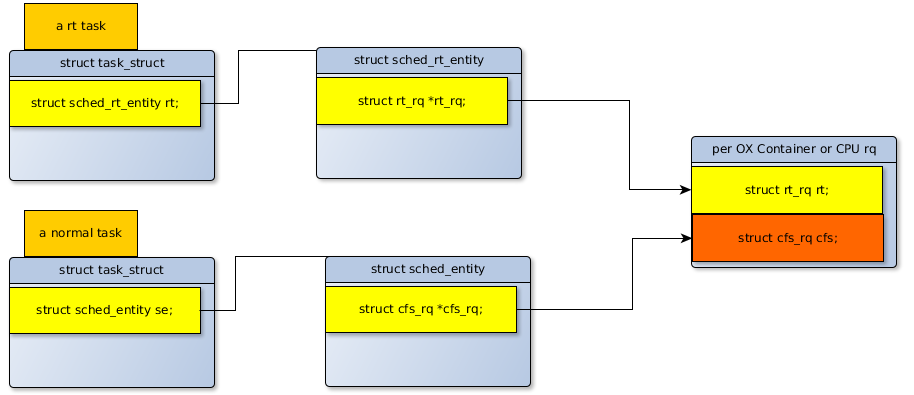
\includegraphics[width=\textwidth]{images/oxc_task_no_tg}
        \caption{New scheduling route for tasks when task group scheduling is not enabled}
        \label{fig:oxc_task_no_tg}
\end{figure}

The first feature of oxc scheduling is that it is compatibe with Linux original
scheduling. Tasks dealt by rt scheduler or cfs can naturally work under the
oxc scheduling system. When there is new scheduling algorithm implemented in
Linux kernel, like the \emph{sched deadline} patch we mentioned before, the
new scheduler has to fullfill details behind scheduling interfaces in 
\texttt{struct sched\_class}. Again, for each shceduling class, they do not
care the interface is passed a per CPU or per container runqueue as the
parameter, and the new scheduling class can also work under oxc scheduling.
So, the ox container structure is open to extension; this is where the name
is from.

Based on per CPU scheduling, each scheduling operation defined in 
\texttt{struct sched\_class} will affect all tasks in the CPU. The
oxc scheduling provides another opportunity to apply a scheduling class in a 
fine grained scale. Now, the scale to apply a scheduler can be controlled 
in the unit of an ox container. 

\section{Movtivation for oxc scheduling framework}
In section \ref{sec:RelatedWork}, we see that based on Linux CPU bandwidth 
control can be applied in the level of single tasks or task groups which 
are shceudled by some policies. Such control can be real-time or non real-time.
One obervation here is that there does not exist a mechanism that can
control CPU bandwidth for all kinds of tasks as a whole.
Such a general control mechanism is the initial consideration of
OXC framework.

Suppose there is an ox container, different schedulers can use it to enqueue,
operate, and dequeue its tasks. If a fraction of CPU bandwidth can be assigned
to this oxc, all kinds of tasks will use it as running on a less powerful
machine. This is the oxc solution to realize CPU bandwidth control as a whole.


\section{Development of OXC scheduling framework}
The oxc framework is still ongoing. Stable codes can be found 
in github\footnote{https://github.com/YIYAYIYAYOUCHENG/linux}.
The oxc framework is not a scheduler, it only interests in CPU bandwidth
control to an oxc, which depends on modular schedulers to use it for 
scheduling tasks.

\subsection{Implementation of ox container structure}
An ox container \texttt{struct oxc\_rq} is implemented in Linux kernel.
An \texttt{struct oxc\_rq} can reserve bandwidth from a CPU using CBS
rules. The CPU reservation for oxc runqueue follows the implementation
of CBS reservation for a rt runqueue in IRMOS framework. 
In the following context, an \texttt{struct oxc\_rq} is also called ox 
container, container, and oxc runqueue for the same meaning. An oxc runqueue
also correspond to a constant bandwidth server in CBS theory. 
\begin{lstlisting}[language=C, caption={\texttt{struct oxc\_rq}},
                        label={oxc_rq}]
struct oxc_rq {
	unsigned long oxc_nr_running;
	inx oxc_throttled;
	u64 oxc_deadline;
	u64 oxc_time;
	u64 oxc_runtime;
	ktime_t oxc_period;
	struct hrtimer oxc_period_timer;
	raw_spin_lock oxc_runtime_lock;
	struct rq rq_;
	struct rq *rq;
	struct rb_node rb_node;
};
\end{lstlisting}

\begin{itemize}
\item \texttt{oxc\_nr\_running} is the number of tasks enqueued in the 
		container's local runqueue. We say these tasks work in 
		the ox container.
\item \texttt{oxc\_throttled} is set when an ox container runs out of
		its budget in a period.
\item \texttt{oxc\_deadline} is current deadline of this ox container,
		which is a server in CBS theory.
\item \texttt{oxc\_time} is currently consumed budget in a period.
\item \texttt{oxc\_runtime} and \texttt{oxc\_period} are CBS parameters:
		\texttt{oxc\_runtime} is maximum budget and 
		\texttt{oxc\_period} is the period.
\item \texttt{oxc\_period\_timer} is timer which will activate at recharging
		points. If at some point, the value of \texttt{oxc\_time} is 
		larger than the value of \texttt{oxc\_runtime}, then
		\texttt{oxc\_throttled} should be set until 
		\texttt{oxc\_period\_timer} fires to recharge the container.
\item \texttt{oxc\_runtime\_lock} guarantee that the timing information of the 
		oxc is updated in a consistant way.
\item \texttt{rq\_} is the local runqueue of the ox container.
\item \texttt{rq} points to a per CPU runqueue and this CPU is where the 
		ox container reserves bandwidth from.
\item \texttt{rb\_node} is used to put an ox quneueu in a red black tree.
		All oxc runqueues reserve bandwidth from the same CPU
		is put in a red black tree associated with this CPU.
		In this tree, an ox container's \texttt{oxc\_deadline} 
		value is used to order nodes.
		runqueue 
\end{itemize}

All oxc runqueues that reserve bandwidth from the same CPU are put in the 
same red black tree, which orders its nodes according to the ox container's
\texttt{oxc\_deadline} value. The one with latest deadline is stored in the
leftmost node. 
\begin{lstlisting}[language=C]
struct oxc_edf_tree {
	struct rb_root rb_root;
	struct rb_node *rb_leftmost;
};
\end{lstlisting}
The pointer \texttt{rb\_leftmost} helps fast access to the latest deadline
ox container in a CPU.

An ox container is responsible for reserving bandwidth from a CPU.
Th \texttt{struct hyper\_oxc\_rq} is defined to reserve bandwidth from
multiple CPUs. 
\begin{lstlisting}[language=C]
struct hyper_oxc_rq {
	cpumask_var_t cpus_allowed;
	struct oxc_rq ** oxc_rq;
};
\end{lstlisting}
\begin{itemize}
\item \texttt{cpus\_allowed} specifies the CPUs that are used to reserve 
				bandwidth.
\item \texttt{oxc\_rq} is an array of ox containers to reserve bandwidth 			
		from CPUs specified in \texttt{cpus\_allowed}.
\end{itemize}

\subsection{Extensions on original data structures}
Extensions are added in some original data structures in order to merge
newly defined data structures in the system. Such extensions are not complex.
\begin{lstlisting}[language=C, caption={Extensions in \texttt{struct rq}}]
struct rq {
	...
	int in_oxc;
	struct oxc_edf_tree oxc_edf_tree;
};
\end{lstlisting}
As the name says, for an ox container's local runqueue, its 
\texttt{in\_oxc} field is set. And \texttt{oxc\_edf\_tree} in a 
per CPU runqueue help locate the ox container's edf tree in a CPU.

In current implementation of oxc framework, reservation is made for 
tasks in a control group. Tasks in a cgroup is represented in the
\texttt{struct task\_group} structure. So extensions also happen inside it.
\begin{lstlisting}[language=C, caption={Extensions in 
						\texttt{struct task\_group}}]
struct task_group {
	...
	struct hyper_oxc_rq *hyper_oxc_rq;
	int oxc_label;
};
\end{lstlisting}
Because tasks in a group can span multiple CPUs, the hyper container is
used to reserve bandwidth for it.
If a task group runs above a hyper oxc, its \texttt{hyper\_oxc\_rq} points 
to the hyper container; otherwise, this field is NULL.
When you associate a hyper container to a task group, its non oxc decendant 
task groups will also be associated with this hyper container, the 
\texttt{oxc\_label} field is used to specify this kind of sub task groups.

If a task runs in a ox container, it is called an oxc task. 
In section \ref{sec:design_oxc_scheduling}, we show how to direct a task
to the runqueue it runs above, which may be a per CPU or container one.
A further check of the runqueue's \texttt{in\_oxc} field can tell us
whether a task is an oxc task or not. Consider that such ''is that an oxc
task?'' is often used in the framework, a \texttt{is\_oxc\_task} field is
added in \texttt{struct task\_struct} for efficient reason.
\begin{lstlisting}[language=C, caption={\texttt{is\_oxc\_task} field in 
						\texttt{struct task\_struct}}]
struct task_struct {
	int is_oxc_task;
	...
};
\end{lstlisting}
When a task runs in an ox container, this field is set.

\subsection{The point to direct a task to a per ox container runqueue}
To schedule a task in a per oxc runqueue, the first thing is to associate
this task with the local runqueue of an oxc. To understand this, let's
first see how the system associate a task to a runqueue in mainline Linux,
where there is only per CPU runqueue concepts. 
\begin{lstlisting}[language=C, 
	caption={To associate a task with a runqueue in original Linux}]
void set_task_rq(struct task_struct *p, unsigned int cpu)
{
#ifdef CONFIG_FAIR_GROUP_SCHED
        p->se.cfs_rq = task_group(p)->cfs_rq[cpu];
        p->se.parent = task_group(p)->se[cpu];
#endif

#ifdef CONFIG_RT_GROUP_SCHED
        p->rt.rt_rq  = task_group(p)->rt_rq[cpu];
#endif
}
\end{lstlisting}
When task group scheduling is enabled, each task is directed to its task group.
This correspond to the first part of scheduling route. The second part of 
the scheduling route from task group to per CPU runqueue is done when the 
task group is created. Figure \ref{tg_creation} shows the hint how a 
task group joins the scheduling route during its creation.
\begin{figure}[htbp]
        \centering
        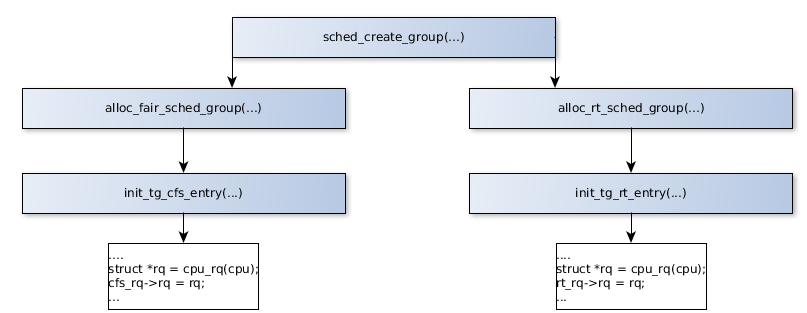
\includegraphics[width=\textwidth]{images/tg_creation}
        \caption{The creation of a task group in original Linux}
        \label{fig:tg_creation}
\end{figure}
In case that task group scheduling is not enabled, recall the scheduling path
where the \texttt{task\_rq} leads a task to its per CPU runqueue directly.

Now, we have seen the point a task joins the scheduling path in original Linux.
It's time to see the scenario after per oxc runqueue is imported in Linux.
Still, \texttt{set\_task\_rq} is the point to associate a task with a 
runqueue, per CPU or per oxc now.
\begin{lstlisting}[language=C, 
        caption={To associate a task with a runqueue under oxc framework}]
void set_task_rq(struct task_struct *p, unsigned int cpu)
{
        struct task_group *tg = task_group(p);

#ifdef CONFIG_FAIR_GROUP_SCHED
        p->se.cfs_rq = tg->cfs_rq[cpu];
        p->se.parent = tg->se[cpu];
#else
        if(!tg->hyper_oxc_rq)
                p->se.cfs_rq = &cpu_rq(cpu)->cfs;
        else
                p->se.cfs_rq = &tg->hyper_oxc_rq->oxc_rq[cpu]->rq_.cfs;
#endif

#ifdef CONFIG_RT_GROUP_SCHED
        p->rt.rt_rq  = tg->rt_rq[cpu];
        p->rt.parent = tg->rt_se[cpu];
#else
        if(!tg->hyper_oxc_rq)
                p->rt.rt_rq = &cpu_rq(cpu)->rt;
        else
                p->rt.rt_rq = &tg->hyper_oxc_rq->oxc_rq[cpu]->rq_.rt;
#endif
        if (task_rq_oxc(p)->in_oxc == 1)
                p->is_oxc_task = 100;
        else
                p->is_oxc_task = 0;
}
\end{lstlisting}
                                                  
When task group scheduling is enabled, there is no difference in cases of 
original Linux and oxc enabled Linux. The interesting part happens when 
task group scheduling is not set. This time, given the task group is associated
with a hyper oxc or not, the task is drected to a per CPU or oxc runqueue. This 
corresponds the scheduling route in figure \ref{fig:oxc_task_no_tg}. In 
the end of the method, \texttt{is\_oxc\_task} is configured. 
\texttt{task\_rq\_oxc} tracks the shceduling route to find the runqueue.

In oxc enabled Linux, a task group can be associated with a hyper oxc and
the runqueues it contains in three cases:1. when it is created, its parent is 
associated with a hyper oxc 2. the task group is explicitly attached to
a hyper oxc 3. one its acendant task group is attached to a hyper oxc.
\begin{figure}[htbp]
        \centering
        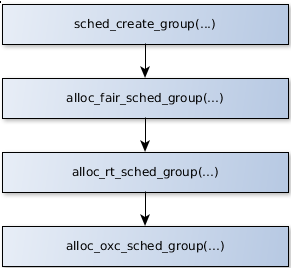
\includegraphics[height=0.25\textheight,width=0.5\textwidth]{images/tg_creation_oxc}
        \caption{The creation of a task group in oxc enabled Linux}
        \label{fig:tg_creation_oxc}
\end{figure}

\begin{lstlisting}[language=C,
        caption={OXC scheduling related initilization 
					during task group creation}]
int alloc_oxc_sched_group(struct task_group *tg, struct task_group *parent)
{
        int i;

        tg->hyper_oxc_rq = parent->hyper_oxc_rq;
        if( parent->hyper_oxc_rq) {
                for_each_possible_cpu(i) {
#ifdef CONFIG_FAIR_GROUP_SCHED
                        tg->cfs_rq[i]->rq =
                                &tg->hyper_oxc_rq->oxc_rq[i]->rq_;
                        if( !parent->se[i] && tg->se[i])
                                tg->se[i]->cfs_rq =
                                      &tg->hyper_oxc_rq->oxc_rq[i]->rq_.cfs;
#endif
#ifdef CONFIG_RT_GROUP_SCHED
                        tg->rt_rq[i]->rq =
                                &tg->hyper_oxc_rq->oxc_rq[i]->rq_;
                        if( !parent->rt_se[i] && tg->rt_se[i])
                                tg->rt_se[i]->rt_rq =
                                       &tg->hyper_oxc_rq->oxc_rq[i]->rq_.rt;
#endif
                }
                tg->oxc_label = 100;
        }
        else
                tg->oxc_label = 0;

        return 1;
}
\end{lstlisting}
\texttt{alloc\_oxc\_sched\_group} deals with oxc related initialization when a 
new task group is created. At first, the a newly created task group will inherit
its parent task group's hyper container. If the parent is an oxc task group, it
directs its scheduling path to the per oxc runqueue. And the \texttt{oxc\_label}
for such child oxc task group is 100.

A task group can direct to a OXC local runqueue explicitly through 
\texttt{init\_tg\_cfs\_entry\_oxc} and \texttt{init\_tg\_rt\_entry\_oxc}.
Let's have a look at \texttt{init\_tg\_cfs\_entry\_oxc} as an example.
\begin{lstlisting}[language=C, caption={To explicitlt direct a task group 
						to an OXC local runqueue}]
static void init_tg_cfs_entry_oxc(struct task_group *tg,
					struct cfs_rq *cfs_rq,
					struct sched_entity *se, int cpu,
					struct sched_entity *parent,
					struct oxc_rq *oxc_rq)
{
	struct rq *rq = rq_of_oxc_rq(oxc_rq);
	init_tg_cfs_entry(tg, cfs_rq, se, cpu, parent);
	tg->cfs_rq[cpu]->rq = rq;
	if( !parent && se)
		se->cfs_rq = &rq->cfs;
} 
\end{lstlisting}
Brief explaination on the parameters:
\begin{itemize}
\item \texttt{tg} is the task group to be dealt with.
\item \texttt{cfs\_rq} is the cfs runqueue the cfs entity of this task
		group is enqueued. 
\item \texttt{se} is the cfs entity that represents \texttt{tg}.
\item \texttt{cpu} specifies the cfs\_rq pointer inside \texttt{tg} that
		will be redirected.
\item \texttt{parent} points to the parent cfs scheduling entity.
\item \texttt{oxc\_rq} contains the destinated runqueue. 
\end{itemize}
As for codes, \texttt{rq\_of\_oxc\_rq} first returns the OXC local runqueue.
\texttt{init\_tg\_cfs\_entry} initialize CFS related work for \texttt{tg}.
Then, \texttt{tg} directs its local \texttt{cfs\_rq} for containing 
tasks on \texttt{cpu} to the per OXC runqueue just got. From now on, cfs 
tasks and task groups under \texttt{tg} work in the scheduling route which
will lead them to an OXC local runqueue. By directing a hierarchy of task
group to an OXC, there is a top group, which will be enqueud in the per
OXC runqueue's embedded cfs runqueue directly.

Now we see how to direct a task group to a per OXC runqueue when task group
scheduling is enabeld. In the whole procedure, tasks under this group is 
untouched.

\subsection{Run tasks under OXC scheduling framework}
As long as per OXC runqueue joins the scheduling route, the scheduling 
of tasks is compatible with modular schedulers in Linux. For an OXC task,
just pass the task itself and its OXC local runqueue, instead of per CPU
runqueue, to its corresponding scheduling class. And the scheduler will
behave as usual.

Because we consider reserving CPU bandwidth for an OXC runqueue, necessary
operations are performed before relaying a task to its modular scheduler.
Still scheduling details are not the framework's interest. 

In order to fullfill real time guarantee, oxc tasks are always privileged
to non oxc tasks. Amg oxc tasks inside a container, the priority relation
is the same as in Linux. The ox container itself can be considered as a 
virtual Linux system.

\subsubsection{To obtain the runqueue of a task}
A method \texttt{tas\_rq\_oxc} is used to obtain the runqueue of a task.
The runqueue retuned can be oxc local runqueue or per CPU one depending
that whether the task is inside a container.
\begin{lstlisting}[language=C]
struct rq* rq_of_task(struct task_struct *p)
{
	struct rq *rq;

#ifdef CONFIG_FAIR_GROUP_SCHED
	rq = p->se.cfs_rq->rq;
#else
	rq = task_rq_fair_oxc(p);
#endif
	return rq;
}
\end{lstlisting}
For any task, it has both cfs scheduling entity and rt entity. So the
rt and cfs scheduling routes both exists for a task. Here, we utilize
the cfs scheduling route. Given \texttt{CONFIG\_FAIR\_GROUP\_SCHED}
is set or not, the corresponding scheduling routes are explored to
track the runqueue.

\subsubsection{To enqueue an oxc task}
When an oxc task arrives, besides enqueue it in the oxc local runqueue,
the ox container information may be updated if necesary.
\begin{lstlisting}[language=C]
void enqueue_task_oxc(struct rq *rq, struct task_struct *p, int flags)
{
	struct oxc_rq *oxc_rq = oxc_rq_of_task(p);
	struct rq *rq_ = rq_of_oxc_rq(oxc_rq);

	/* Update the local runqueue' clock. */
	update_rq_clock(rq_);

	/*
	* Enqueue the task into the local runqueue
	* by its scheduling class.
	*/
	p->sched_class->enqueue_task(rq_, p, flags);

	inc_oxc_tasks(p, oxc_rq);
	enqueue_oxc_rq(oxc_rq);
}
\end{lstlisting}
\texttt{oxc\_rq\_of\_task} tracks the scheduling route and returns the ox
container of an oxc task. Then local runqueue's time information is updated.
Although the ox container does not care about scheduling details of tasks 
inside it, tasks are enqueued in its local runqueue and may rely the
runqueue's time information. Then we see all scheduling details are dealt 
by a task's scheduling class as the \texttt{enqueue\_task} of the
scheduling class is called with the task and local runqueue.
The \texttt{inc\_oxc\_tasks} method is simple.
\begin{lstlisting}[language=C]
static inline void inc_oxc_tasks(struct task_struct *p, struct oxc_rq *oxc_rq)
{
        oxc_rq->oxc_nr_running ++;
}
\end{lstlisting}

Until now, the oxc task has been put in the local runqueue. The coming of an
oxc task in a container may change the relation among ox containers in the
same edf tree. This is the work of \texttt{enqueue\_oxc\_rq} method. 
\begin{lstlisting}[language=C]
static void enqueue_oxc_rq(struct oxc_rq *oxc_rq)
{
        int on_rq;

        on_rq = oxc_rq_on_rq(oxc_rq);

        BUG_ON(!oxc_rq->oxc_nr_running);
        BUG_ON(on_rq && oxc_rq_throttled(oxc_rq));

        if( on_rq) {
                /* Already queued properly. */
                return;
        }
        /* We do not put a throttled oxc_rq in the edf tree. */
        if( oxc_rq_throttled(oxc_rq))
                return;

        oxc_rq_update_deadline(oxc_rq);
        __enqueue_oxc_rq(oxc_rq);
}
\end{lstlisting}
\texttt{on\_rq} tells if the container \texttt{oxc\_rq} is in a edf tree.
\texttt{BUG\_ON} is a Linux kernel macro. If the condition it checks is 
\texttt{true}, then the kernel will crash! Because we just put a task
in the local runqueue, so the first \texttt{BUG\_ON} should be passed.
When an ox container runs out of its budget, it should be moved from the
edf tree, this is what the second \texttt{BUG\_ON} checks. Now we pass
the two \texttt{BUG\_ONs}. If the \texttt{oxc\_rq} is already on edf 
tree or moved from the tree because of exhausting budget, nothing to
be done. There are two conditions for an ox container outside an edf
tree: it is throttled or it is empty. This means a task just joins
an empty container. Recall the CBS rules ''when a task arrives and 
the server is idle, update the deadline if necessary''. This is what
\texttt{oxc\_rq\_update\_deadline} does. When it comes to CPU reservation,
an ox container corresponds to a constant bandwidth server in CBS theory.
texttt{\_enqueue\_oxc\_rq} is quite a mechanical procesure to put an
oxc runqueue in an edf tree.

\subsubsection{To dequeue an oxc task}
\texttt{dequeue\_task\_oxc} is the opposite method of 
\texttt{enqueue\_oxc\_rq}.
\begin{lstlisting}[language=C]
static void dequeue_task_oxc(struct rq *rq, struct task_struct *p, int flags)
{
        struct rq *rq_ = task_rq_oxc(p);
        struct oxc_rq *oxc_rq = container_of(rq_, struct oxc_rq, rq_);

        /* Update the local runqueue. */
        update_rq_clock(rq_);
        /*
         * Dequeue the task from the local runqueue 
         * by its scheduling class.
         */
        p->sched_class->dequeue_task(rq_, p, flags);

        dec_oxc_tasks(p, oxc_rq);
        dequeue_oxc_rq(oxc_rq);
}
\end{lstlisting}
The structure of \texttt{dequeue\_task\_oxc} are the same as 
\texttt{enqueue\_task\_oxc}: local runqueue's time information is updated,
local runqueue and task is relayed to the corresponding scheduler, 
and the task number is decreased. When an oxc task leaves the container,
it is the time to check if the oxc is empty or not, which is done in
\texttt{dequeue\_oxc\_rq}.
\begin{lstlisting}[language=C]
static void dequeue_oxc_rq(struct oxc_rq *oxc_rq)
{
        int on_rq;

        on_rq = oxc_rq_on_rq(oxc_rq);
        /*
         * Here we do not expect throttled oxc_rq to be in the edf tree.
         * Note that when an oxc_rq exceeds its maximum budget,
         * it is dequeued via sched_oxc_rq_dequeue().
         */
        BUG_ON(on_rq && oxc_rq_throttled(oxc_rq));
        /* 
         * If an oxc_rq is not in the edf tree, it should be throttled or 
         * have no tasks enqueued.
         */
        BUG_ON(!on_rq && !oxc_rq_throttled(oxc_rq) && !oxc_rq->oxc_nr_running);

        if( on_rq && !oxc_rq->oxc_nr_running) {
                /* Dequeue the oxc_rq if it has no more tasks. */
                __dequeue_oxc_rq(oxc_rq);
                return;
        }
}
\end{lstlisting}
The comments are explainable enough. \texttt{\_\_dequeue\_oxc\_rq} removes 
a oxc runqueue from the edf tree.

\subsubsection{To check the preemption}
When a task wakes up from sleeping or is created, the scheduler will check 
if it can preempt current running task in the same CPU. If the current task
is an oxc task and the waking task is not an oxc task, the later cannot
preempt the current one. If both are non oxc tasks, Linux already has methods
to check. So here we only interest in the case when the waking task is an
oxc task.\\

\begin{lstlisting}[language=C]
static inline int
check_preempt_oxc_rq(struct task_struct *curr, struct task_struct *p, int flags)
{
        struct oxc_rq *oxc_rq = oxc_rq_of_task(p);
        struct oxc_rq *oxc_rq_curr = oxc_rq_of_task(curr);
        const struct sched_class *class;

	if(oxc_rq_throttled(oxc_rq)
		return 0;
        /* 
         * Tasks from a unthrottled oxc_rq always has a higher priority 
         * than non oxc tasks.
         */
        if( !oxc_rq_curr)
                return 1;

        /* Both p and current task are in the same oxc_rq. */
        if( oxc_rq_curr == oxc_rq) {
                if( p->sched_class == curr->sched_class) 
                        curr->sched_class->check_preempt_curr(
                                      &oxc_rq->rq_, p, flags);
                else {
                        for_each_class(class) {
                                if( class == curr->sched_class)
                                        break;
                                if( class == p->sched_class) {
                                        resched_task(curr);
                                        break;
                                }
                        }
                }

                return 0;
        }

        /* p and current tasks are oxc tasks from different ox containers. */
        return oxc_rq_before(oxc_rq, oxc_rq_curr);
}
\end{lstlisting}
\texttt{curr} and \texttt{p} are the current task and wakeing task respectively.
If task \texttt{p}'s container is throttled, it cannot preempt currently running task.
Otherwise, if \texttt{curr} is not an oxc task, \texttt{p} has higher priprity and
preempt \texttt{curr}. When two tasks are contained in the same oxc runqueue: if 
they are even in the same scheduling class, it's the modular scheduler's responsibility
to decide given; otherwise, the task whose scheduling class has higher priority in the
scheduler chain is chosen to run. In the last case, they two are from different 
containers. Now, \texttt{oxc\_rq\_before} checks if a contaienr's deadline is before
another's deadline. The one with smaller deadline will run. 

\subsubsection{To pick up an oxc task}
When to pick a most eligible task to run, oxc tasks should be checked first.
If there is no eligible oxc tasks, then non oxc tasks are considered.
\texttt{pick\_next\_task\_oxc} is responsible for choosing the most 
eligible oxc task in a CPU.
\begin{lstlisting}[language=C]
static struct task_struct* pick_next_task_oxc(struct rq *rq)
{
        struct oxc_rq *oxc_rq;
        struct rq *rq_;
        struct task_struct *p, *curr;
        const struct sched_class *class;
        /* This clock update is necessary! */
        update_rq_clock(rq);
        update_curr_oxc_rq(rq);
        oxc_rq = pick_next_oxc_rq(rq);
        if( !oxc_rq)
                return NULL;

        rq_ = rq_of_oxc_rq(oxc_rq);

        update_rq_clock(rq_);

        for_each_class(class) {
                if( class != &idle_sched_class) {
                        p = class->pick_next_task(rq_);
                        if( p) {
                                rq_->curr = p;
                                return p;
                        }
                }
        }

        return NULL;
}
\end{lstlisting}
There are one thing to note here: not only local runqueue's clock
is updated, but also the per CPU runqueue's clock is updated here.
This is because the reservation time of an ox container is counted
using the per CPU runqueue's clock and to keep the clock on time
for the container's use, here it is updated. 
\texttt{pick\_next\_oxc\_rq} picks the ox runqueue with latest 
deadline in a CPU. And along the scheduling class chain, each
scheduler uses its own way trying to find the most eligible
task in the local runqueue.
Another import method here is \texttt{update\_curr\_oxc\_rq}.
The budget comsumption really happens here.
\begin{lstlisting}[language=C]
static void update_curr_oxc_rq(struct rq *rq)
{
        struct task_struct *curr = rq->curr;
        struct oxc_rq *oxc_rq = oxc_rq_of_task(curr);
        u64 delta_exec;
        /*
         * If current task is not oxc task, simply return.
         */
        if( !oxc_rq)
                return;

        delta_exec = rq->clock - oxc_rq->oxc_start_time;
        oxc_rq->oxc_start_time = rq->clock;
        if( unlikely((s64)delta_exec < 0))
                delta_exec = 0;

        raw_spin_lock(&oxc_rq->oxc_runtime_lock);

        oxc_rq->oxc_time += delta_exec;
        if( sched_oxc_rq_runtime_exceeded(oxc_rq)) {
                resched_task(curr);
        }

        raw_spin_unlock(&oxc_rq->oxc_runtime_lock);
}
\end{lstlisting}
\texttt{update\_curr\_oxc\_rq} updates the runtime information of 
an oxc runqueue. If the budget in current period is exhausted, the
current task needs to be resched. the local spinlock 
\texttt{oxc\_runtime\_lock} protects the update of runtime from
interleave.
\begin{lstlisting}[language=C]
static int sched_oxc_rq_runtime_exceeded(struct oxc_rq *oxc_rq)
{
        u64 runtime = sched_oxc_rq_runtime(oxc_rq);
        u64 period = sched_oxc_rq_period(oxc_rq);

        /* 
         * If the runtime is set as 'RUNTIME_INF',
         * the ox container can run without throttling.
         */
        if( runtime == RUNTIME_INF)
                return 0;

        /* 
         * If the runtime to be larger the the period,
         * the ox container can run without throttling.
         */
        if( runtime >=period)
                return 0;

        /* There is still budget left. */
        if( oxc_rq->oxc_time < runtime)
                return 0;
        /* 
         * The reservation in a period has been exhausted,
         * to set the throttling label, remove the oxc_rq
         * from the edf tree and start the recharging timer.
         */
        else {
                oxc_rq->oxc_throttled = 1;
                sched_oxc_rq_dequeue(oxc_rq);
                start_oxc_period_timer(oxc_rq);

                return 1;
        }
}
\end{lstlisting}
Inside \texttt{sched\_oxc\_rq\_runtime\_exceeded}, at first
a series of non exceeded conditions are checked, which is 
easy to understand. The last \emph{else} statement deals with
the case tha tthe container is throttled: the \texttt{oxc\_throttled}
label is set, the oxc runqueue is removed from the edf tree and 
the timer is set and will fire at the next deadline to recharge the 
budget.

\subsubsection{put\_prev\_task operation}
The scheduling operation is called when the currently running task is
possible to be replaced. It performs some conclusion work for the task.
Although the currently running task may keep running without being
preempted. If currently running task is an oxc task, when 
\texttt{put\_prev\_task} is called, this is also a point to update 
the ox container information. 
\begin{lstlisting}[language=C]
static void put_prev_task_oxc(struct rq* rq, struct task_struct *p)
{
        struct rq *rq_ = task_rq_oxc(p);

	update_rq_clock(rq_);
        update_curr_oxc_rq(rq);

        p->sched_class->put_prev_task(rq_, p);
}
\end{lstlisting}
Now, when a \texttt{put\_prev\_task} operation is needed and the
currently running task is an oxc task, instead of calling the 
\texttt{put\_prev\_task} defined in a scheduling class directly, our
\texttt{put\_prev\_task\_oxc} encapsulation will be called first then
ox container local runqueue and current task will be relayed to
the corresponding scheduler.

\subsubsection{set\_curr\_task operation}
The above \texttt{put\_prev\_task} is the last scheduling operation before 
a task gives up a CPU (of course, if it is chosen again immediately, it
can still occupy the CPU). The \texttt{set\_curr\_task} is the first 
scheduling operation a task performs when it is chosen to use the CPU.
If the newly chosen task is an oxc task, it is also the point to prepare
the ox container for time updating.
\begin{lstlisting}[language=C]
static void set_curr_task_oxc(struct rq *rq)
{
        struct task_struct *curr = rq->curr;
        struct rq *rq_ = task_rq_oxc(curr);
        struct oxc_rq *oxc_rq;

        oxc_rq = container_of(rq_, struct oxc_rq, rq_);

        oxc_rq->oxc_start_time = oxc_rq->rq->clock;

        update_rq_clock(rq_);
        curr->sched_class->set_curr_task(rq);
}
\end{lstlisting}
One thing to note is that inside this encapsulation, the per CPU runqueue
parameter is passed to the task's corresponding scheduling class. This is
because \texttt{set\_curr\_task} operation updates the infomation in the 
scheduling route except for the runqueue itself. So, there is no difference
to pass which runqueue. The real reason is that, there is a possible
insconsistent state. Initially, the current task in ox container local
runqueue is NULL\footnote{This will be fixed in future work}, which is not 
a special idle task from scheduling class \texttt{sched\_idle}. Because
\texttt{set\_curr\_task} is called even before the task is enqueued in the
runqueue( maybe oxc local one). And this will cause problems.

\subsubsection{task\_tick operation}
The \texttt{task\_tick} operation is the most frequently called scheduling 
operation and is used to update the task's timing information. So, if
the task parameter in this method is oxc type, this is the point to
update the confainer's information and local runqueue's clock.
\begin{lstlisting}[language=C]
static void task_tick_oxc(struct rq *rq, struct task_struct *p, int queued)
{
        struct rq *rq_ = task_rq_oxc(p);

        update_curr_oxc_rq(rq);
        update_rq_clock(rq_);

        p->sched_class->task_tick(rq_, p, queued);
}
\end{lstlisting}

\subsection{SMP support in oxc framework}
An ox container based scheduling system on a CPU has no difference with the 
per CPU based scheduling system. Each ox container works independently and
they are arranged in one hyper container. For a hyper container, tasks are
partitioned to each ox container and task migration or load balancing between 
different ox contaienrs in a hyper container are not realized now.

\subsection{User interfaces provided with OXC framework}
Currently, oxc framework provides users with cgroup interfaces.
The CPU reservation functionality is realized through \emph{cpu} cgroup 
subsystem. This \emph{cpu} cgroup subsystem is for CPU bandwidth control
in Linux. RT throttling, fairness group scheduling and CFS bandwidth control
are all realized through it. The following describes how to use the OXC 
framework and the CPU number is assumed to be 2.

To mount the \emph{cpu} cgroup subsystem(in directory /cgroup):
\begin{lstlisting}
	#mount -t cgroup -ocpu none /cgroup
\end{lstlisting} 
To create a cgroup for CPU reservation :
\begin{lstlisting}
	#mkdir -p /cgroup/cg
\end{lstlisting}
Observe the files inside \texttt{/cgroup/cg} directory, there are one
new file \texttt{cpu.oxc\_control} which is the interface to control
CPU bandwidth in oxcframework. However, if one tries to see the content
of this file:
\begin{lstlisting}
	#cat /cgroup/cg/cpu.oxc_control
\end{lstlisting}
It will display nothing. This is because by default the oxc reservation
is disabled initially until the reservation is triggered for the first 
time. The reservation is triggerred by setting reservation parameters.
To reserve bandwidth in a CPU, three parameters should be specified:
CPU number, maximum budget and period. For example:
\begin{lstlisting}
	#echo 0 100000/1000000 1 20000/500000 > cg/cpu.oxc_control
\end{lstlisting}
This command reserve 100ms every 1s on CPU 0 and 20ms every 500ms on CPU 1
to cgroup \texttt{cg}. 0 and 1 are CPU numbers. 100000 and 20000 are maximum
budgets and 1000000 and 500000 are periods. The unit for budget and period
value is millisecond. This follows the convention in \emph{cpu} cgroup
subsystem. So tasks inside this cgroup and its further sub cgroups will
run using the above reserved CPU bandwidth. Now we can say \texttt{cg} is
contained in a hyper ox container.

To ''cat'' the content of the \texttt{cpu.oxc\_control} interface under
directory \texttt{/cgroup/cg}:
\begin{lstlisting}
	#cat /cgroup/cg/cpu.oxc_control
\end{lstlisting}
The above parameters set will be displayed:
\begin{lstlisting}
	0 100000/1000000 1 20000/500000
\end{lstlisting}

Reservation parameters can be configured in the same way. Furthermore,
there is no need to configure reservation parameters for two CPUs at 
the same time. Suppose in some point, users decide to decrease the 
reservation from CPU 1, they can simply use the following command.
\begin{lstlisting}
	#echo 1 20000/1000000 > cg/cpu.oxc_control
\end{lstlisting}
The reservation on CPU 1 is dereased to 20ms every 1s and the reservation
on another CPU is not interfered. 

To create a sub cgroup for cgroup \texttt{cg}:
\begin{lstlisting}
	#mkdir -p /cgroup/cg/cg_0
\end{lstlisting}
The cgroup \texttt{cg\_0} is contained in the same hyper container as
its parent. Try to ''cat'' the \texttt{/cgroup/cg/cg\_0/cpu.oxc\_control}: 
\begin{lstlisting}
	#cat /cgroup/cg/cg\_0/cpu.oxc\_control}
\end{lstlisting}
An error message will be returned. This is because for a cgroup family
contained in a hyper container, only the top cgroup has the right to 
browse and modify reservation parameters.

People can move tasks to cgroup \texttt{cg} and texttt{cg\_0}. For example
\begin{lstlisting}
	#echo 1982 > cg/tasks
	#echo 1983 > cg\_0/tasks
	...
\end{lstlisting}
This moves task with \texttt{pid} 1982 and 1983 to cgroup \texttt{cg} and
\texttt{cg\_0} respectively. Tasks can be rt tasks or normal tasks. All 
tasks inside an ox container behave as working on a virtual Linux system
and utilize the reserved bandwidth. Note here we use ''ox container'', not
''hyper ox container'', because in temporary iplementation, tasks inside
a hyper ox container are partitioned into each CPU. 

The oxc tasks can move between different cgroups contained in the same 
hyper container. They can move between ox containers and hyper containers.
They can also leave an ox container and return to a non oxc task.


Until now, how to reserve CPU bandwidth under oxc framework is introduced.
Now let's see how to distribute the reserved CPU power.
ALthough users cannot browse reservation parameters in cgroup
\texttt{cg\_0}, they can indeed set reservation parameters for 
\texttt{cg\_0}, which will trigger reserved power redistribution.
\begin{lstlisting}
	#echo 0 100000/2000000 1 20000/1000000 > cg/cpu.oxc_control
\end{lstlisting}
After this, a new hyper container with reservation parameters
1000000/1500000 on CPU 0 and 20000/1000000 on CPU 1 will be created
and \texttt{cg\_0} and its decendant cgroups will be associated with
it. Now, although \texttt{cg} and \texttt{cg\_0} are still in the same
hierarchy in the cgroup directory observation, they are indeeded contained
in two different hyper containers.
The ideal effct of the above command should also include that the reserved
bandwidth by \texttt{cg} need to decrease the same vaue as distributed to
\texttt{tg\_0}. This behaviour is still missed in current prorotype 
implementation of oxc framework. Yet this is indeed implementable.
Also, the total reserved bandwidth in the system should not be more one in
each CPU; this condition test is not realised either.

\subsection{Cooperation with scheduling mechanisms inside Linux}
When \texttt{CONFIG\_FAIR\_GROUP\_SCHED} and \texttt{CONFIG\_RT\_GROUP\_SCHED}
are not set; that is, task grouping is not enabled. Tasks work in an ox container
just as the oxc scheduling theory explains. In fact, in this case, oxc framework
can work as RT throttling and CFS bandwidth control in a real time behaviour.
The result of IRMOS real time scheduler can also be achieved by our framework.
Consider future scheduling classes that are possible to be merged in Linux kernel.
For example deadline tasks in \texttt{schedule\_deadline} patch, they do not
have task group scheme. The oxc framework provide them a real time way to group
their tasks and because of the ''open to extension'' feature for ox container, to
merge them with oxc framework is natural.

When fairness task group shceduling is enabled, task groups under the same 
hyper ox container follow the rules of fairness task grouping and share the 
reserved CPU power. Fairness task group scheduling is applied in different 
areas independently: each hyper ox container is an area, outside ox containers
there is the other area. Inside one hyper ox container, bandwidths are reserved
and task groups inside this hyper ox container share the reserved computation
power arrording to the fairness task group scheduling rules. 

When \texttt{CONFIG\_RT\_GROUP\_SCHED} is set, RT throttling is enabled.
Let's first analyze the possible result when RT throttling is applied in
a hyper ox container. Suppose inside an container, $Q/T$ is the 
bandwidth reserved from the CPU and RT throttling sets parameters as 
$Q^{'}/T^{'}$ and $Q^{'}/T^{'} \le Q/T$. The ideal behaviour for such an
ox container would be : the container distributes reserved CPU power 
to tasks inside it; and rt tasks inside a group will be throttled when
$Q^{'}$ units of CPU cycles are exhausted in period $T^{'}$, then non
rt tasks can run. However, there are also other possibilities.
For example, $Q^{'}/T^{'} = 1/10$ and $Q/T = 10/50$. Suppose there
are other higher priority containers in the same CPU and in one period 
the example container get the right to use the CPU on the last 10 units
of CPU cycles in its period. RT tasks inside thsi container immediately,
yet after one unit, they are throttled and has to give up. So, during the
whole period, rt tasks only run 1 unit over 50 unit of CPU cycles. The RT
throttling result inside a hyper ox container is not stable. 
Even we set the period parameter in RT throttling the same as its 
container's, because of RT throttling using different \emph{hrtimer} 
from oxc reservation, the unsyhcronization between can also cause even more 
complex situation.

In a word, to merge RT throttling directly inside container is not efficient.
One possible solution is to count the time consumption in rt throttling using 
the same timer, this basically means to implement a copy of RT throttling 
in oxc framework itself. In such case, if some constraints are put, like
the RT throttling period should equal to its container's period, we can
expect predictable behaviour.
Another solution is simply disable RT throttling inside container, because
oxc scheduling framework itself can perform the same result in a real time
way as RT throttling. 
In current implementation, solution one is used when 
\texttt{CONFIG\_RT\_GROUP\_SCHED} is set, and result is not satisfiable.

The behaviour when CFS bandwidth control is enabled. We predict the behaviour
should be similiar to what we see in RT throttling case.

Among cgroup subsystems, there is one \texttt{cpuset} also effecting scheduling
behaviour in a cgroup.
After \texttt{cpuset} cgroup subsystem is mounted in a cgroup, there is an 
interface \texttt{cpuset.cpus} appearring in the dorectory. Which can control
which CPU the tasks inside this cgroup can use.
For example, 
\begin{lstlisting}
	#echo 1 > cpuset.cpus
\end{lstlisting}
This will result tasks inside this cgroup can only run on CPU 1.
In oxc scheduling framework, we have the concept of hyper ox container, which 
control which CPUs tasks inside hyper container can run. So, this idea is
compatible with \texttt{cpuset} cgroup subsystem. However, until now the two
work independently; future work to bridge the two will make the system more
efficient.
